\chapter{\ifproject%
\ifenglish Experimentation and Results\else การทดลองและผลลัพธ์\fi
\else%
\ifenglish System Evaluation\else การประเมินระบบ\fi
\fi}
\begin{mypara}
    \indent การทดลองและประเมินของผลระบบ DeSS-T แบ่งออกเป็น 2 ส่วนหลัก คือ การทดสอบความถูกต้องแม่นยำของระบบจำลอง 
    และการประเมินความพึงพอใจและรับข้อเสนอแนะการใช้งานจากผู้ใช้จริง โดยมีรายละเอียดและผลการดำเนินงานดังนี้
\end{mypara}


\section{การวัดและประเมินความถูกต้องแม่นยำของระบบจำลอง}
\begin{mypara}
    \indent ในส่วนนี้เป็นการทดสอบเพื่อให้แน่ใจว่าระบบจำลองที่พัฒนาขึ้น 
    สามารถสะท้อนพฤติกรรมของระบบขนส่งได้อย่างเหมาะสม โดยจะแบ่งออกเป็น 2 ส่วน คือ
\end{mypara}
\subsection{การประเมินความถูกต้อง}
\begin{mypara}
    \indent การประเมินความถูกต้องมุ่งเน้นไปที่การตรวจสอบว่า
    ระบบสามารถประมวลผลได้ตรงตามตรรกะและข้อมูลนำเข้า โดยแบ่งการทดลองเป็น 2 รูปแบบ ดังนี้
\end{mypara}
    \begin{enumerate}
        \item การประเมินความถูกต้องของระบบจำลอง
            \begin{mypara}
                \indent เพื่อดำเนินการตรวจสอบความถูกต้องของระบบจำลอง โดยมุ่งเน้นการทดสอบ
                เชิงตรรกะว่าระบบสามารถตอบสนองต่อการปรับเปลี่ยนตัวแปรนำเข้าได้สอดคล้องกับ
                พฤติกรรมในความเป็นจริงหรือไม่ การทดลองนี้ใช้วิธีการวิเคราะห์ความอ่อนไหว 
                (Sensitivity Analysis) ผ่านการปรับเปลี่ยน 2 ตัวแปรหลัก คือ 
                ปริมาณผู้โดยสาร (Arrival Rate) และความถี่ในการออกรอบของรถ (Bus Schedule)
                เพื่อสังเกตการเปลี่ยนแปลงของค่าสถิติ 3 ตัวชี้วัด ได้แก่ เวลารอคอยเฉลี่ย
                 (Avg. Waiting Time) ความยาวแถวคอยเฉลี่ย (Avg. Queue Length) 
                 และอัตราการใช้งานรถเฉลี่ย (Avg. Utilization) โดยสรุปผลลัพธ์ได้ดังนี้
            \end{mypara}
                \begin{enumerate}
                    \item \textbf{ผลกระทบจากการปรับเปลี่ยนปริมาณผู้โดยสาร:}
                    จากการทดลองพบว่า เมื่อกำหนดให้ความถี่รถคงที่ การเพิ่มขึ้นของจำนวนผู้โดยสาร
                    ส่งผลโดยตรงต่อค่าสถิติทุกด้าน เช่น ในกรณีที่รถออกรอบน้อย (ทุก 1 ชั่วโมง) 
                    เมื่อผู้โดยสารหนาแน่น (มาทุก 5 นาที) เวลารอคอยเฉลี่ยจะสูงถึง 71.9 นาที 
                    แต่เมื่อผู้โดยสารน้อยลง (มาทุก 20 นาที) เวลารอคอยจะลดลงเหลือ 28.2 นาที
                    ซึ่งการแปรผันของตัวเลขสถิตินี้สะท้อนถึงความถูกต้องของแบบจำลองในการตอบสนองต่ออุปสงค์ที่เปลี่ยนแปลงไป

                    \item \textbf{ผลกระทบจากการปรับเปลี่ยนความถี่การออกรอบของรถ:} 
                    การเพิ่มความถี่ของรถช่วยบรรเทาความแออัดได้อย่างชัดเจน แม้ในสภาวะที่มีผู้โดยสาร
                    หนาแน่น (มาทุก 5 นาที) หากเพิ่มความถี่รถเป็นทุก 10 นาที จะส่งผลให้
                    เวลารอคอยเฉลี่ยลดลงอย่างมีนัยสำคัญเหลือเพียง 4.4 นาที และความยาวแถวคอยลดลง
                    เหลือ 0.4 คน เนื่องจากมีการระบายผู้โดยสารได้รวดเร็วขึ้น
                \end{enumerate}

        \begin{table}[h]
        \centering
        \caption{ตารางสรุปเปรียบเทียบค่าสถิติจากการจำลอง}
        \label{tab:sim_accuracy_results}
        \begin{tabular}{|l|l|c|c|c|}
        \hline
        \textbf{ปริมาณผู้โดยสาร} & \textbf{ความถี่รอบรถ} & \textbf{เวลารอเฉลี่ย (นาที)} & \textbf{แถวคอยเฉลี่ย (คน)} & \textbf{การใช้งานรถ (\%)} \\ \hline
        หนาแน่น (5 นาที) & น้อย (1 ชม.) & 71.9 & 24.9 & 77\% \\ \hline
        น้อย (20 นาที) & น้อย (1 ชม.) & 28.2 & 1.0 & 25\% \\ \hline
        หนาแน่น (5 นาที) & เยอะ (10 นาที) & 4.4 & 0.4 & 16\% \\ \hline
        น้อย (20 นาที) & เยอะ (10 นาที) & 3.9 & 0.1 & 3\% \\ \hline
        \end{tabular}
        \end{table}
        \textbf{วิเคราะห์และสรุปความถูกต้อง:}
        จากผลการทดลองในตารางที่ \ref{tab:sim_accuracy_results} พบว่าผลลัพธ์
        จากระบบจำลองมีแนวโน้มสอดคล้องกับหลักความเป็นจริง
        โดยค่าสถิติจะสูงที่สุดในสภาวะที่มีปริมาณผู้โดยสารสูงและรอบรถน้อย 
        (High Demand / Low Supply) และค่าจะต่ำที่สุดเมื่อผู้โดยสารน้อยและรอบรถมาก 
        (Low Demand / High Supply) การที่ระบบสามารถแสดงผลลัพธ์ ได้อย่าง
        สมเหตุสมผล เป็นการยืนยันว่าระบบการจำลองที่พัฒนาขึ้นมีความถูกต้องเชิงตรรกะ
        และพร้อมสำหรับการนำไปใช้งาน
        \item การประเมินความถูกต้องของผลลัพธ์เชิงสถิติ
            \begin{mypara}
                \indent ได้ทำการทดสอบผ่านระบบจำลองเพื่อเปรียบเทียบกับข้อมูลจริงจากรถขนสนสาธารณะในมหาวิทยาลัยเชียงใหม่
                สายบริการ 2 เส้นทาง ได้แก่ สาย 5 และสาย 7 โดยใช้ข้อมูลในช่วงเวลา 08:00 – 10:00 น. ของวันอังคารและวันศุกร์ 
                นำมาจำลองจำนวน 100 รอบ ผลการทดลองมีรายละเอียดดังนี้
            \begin{itemize}
                \item \textbf{สายบริการ 5:} ให้ค่าความถูกต้องของเวลารอคอยเฉลี่ย 
                (Avg. Waiting Time) อยู่ที่ 94.71\% และอัตราการใช้งานรถเฉลี่ย 
                (Avg. Utilization) อยู่ที่ 92.23\% เนื่องจากสายนี้มีการจัดเก็บข้อมูล
                ที่ครอบคลุมในทุกสถานีอย่างทั่วถึง
                \item \textbf{สายบริการ 7:} ให้ค่าความถูกต้องของเวลารอคอยเฉลี่ย
                อยู่ที่ 75.06\% และอัตราการใช้งานรถเฉลี่ยอยู่ที่ 60.60\% ซึ่งมีค่าต่ำกว่า
       50         สายบริการ 5 อย่างมีนัยสำคัญ สาเหตุหลักมาจากข้อมูลที่จัดเก็บได้ของสาย 7 
                ส่วนใหญ่กระจุกตัวอยู่ที่สถานีกลางเป็นหลัก ในขณะที่สถานีอื่น ๆ มีปริมาณข้อมูลน้อย 
                ส่งผลให้ความถูกต้องโดยรวมของผลลัพธ์เชิงสถิติลดลง
            \end{itemize}
            \begin{figure}[H]
                \centering
                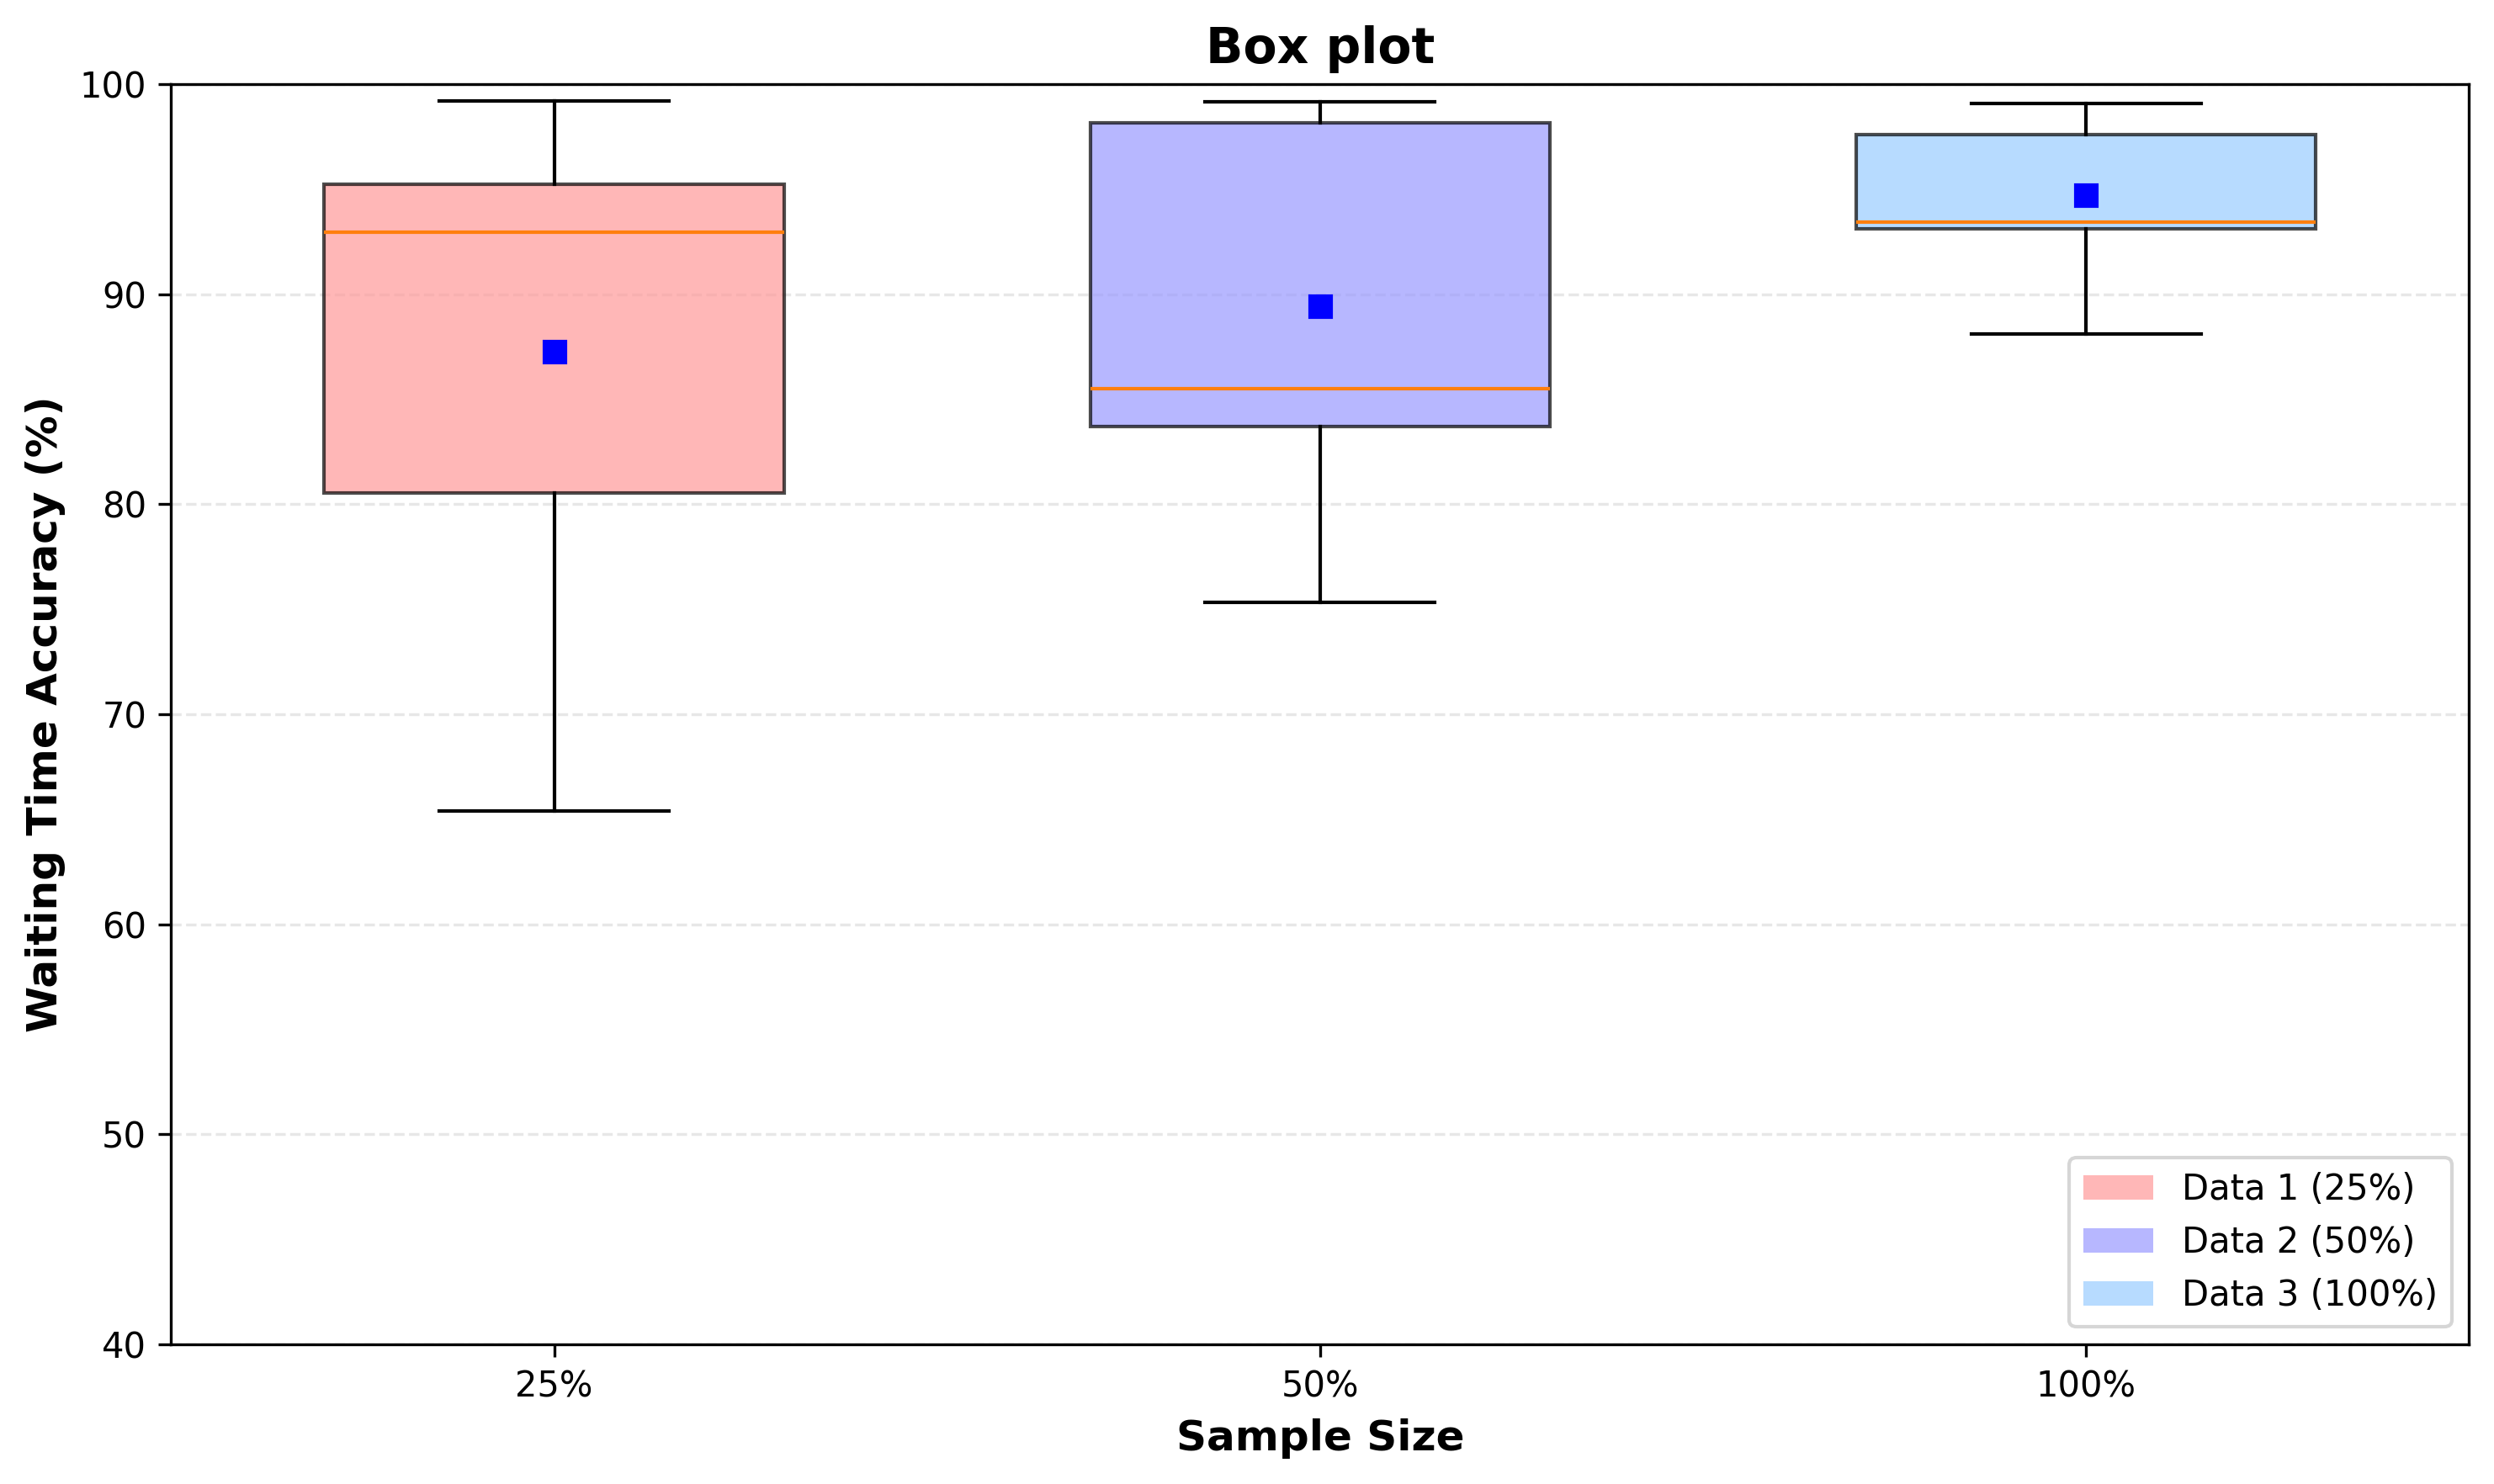
\includegraphics[width=0.60\textwidth,height=0.50\textheight,keepaspectratio]{box plot.png}
                \caption{Box Plot แสดงความแตกต่างของความถูกต้องระหว่างปริมาณข้อมูลนำเข้าที่แตกต่างกัน}
                \label{fig:BoxPlotAccuracy}
            \end{figure}
            \indent นอกจากนี้ ผลการวิเคราะห์ยังแสดงให้เห็นว่าขนาดของกลุ่มตัวอย่าง 
            (Sample Size) มีผลโดยตรงต่อค่าเฉลี่ยความถูกต้อง (Mean Accuracy) 
            โดยเมื่อปริมาณข้อมูลเพิ่มขึ้นจาก 25\% เป็น 50\% และ 100\% ระบบจะสามารถ
            สร้างฟังก์ชันการแจกแจงที่ใกล้เคียงกับความเป็นจริงได้มากขึ้น ส่งผลให้ค่าความ
            ถูกต้องเฉลี่ยเพิ่มสูงขึ้นจาก 87.26\% เป็น 89.43\% และ 94.71\% ตามลำดับจากรูปที่
            \ref{fig:BoxPlotAccuracy}
            \textbf{วิเคราะห์และสรุปความถูกต้อง:}จากการทดลองพบว่าความถูกต้องของระบบจำลองมีความแปรผันตาม 
            ความครอบคลุมและปริมาณ ของข้อมูลนำเข้า โดยในกรณีของสาย 5 พิสูจน์ให้เห็นว่าหากมีการเก็บข้อมูลครบทุกสถานี 
            ระบบจะสามารถทำนายประสิทธิภาพการเดินรถได้แม่นยำสูงกว่า 90\% ในขณะที่กรณีสาย 7 ข้อมูลที่กระจุกตัวเพียงบางจุด
            ไม่สามารถเป็นตัวแทนของระบบทั้งหมดได้ ดังนั้น สรุปได้ว่าความแม่นยำของระบบ DeSS-T จะเกิดขึ้นได้สูงสุดเมื่อ
            ผู้ใช้มีการจัดเก็บข้อมูลอุปสงค์ของผู้โดยสารที่กระจายตัวครอบคลุมทุกจุดบริการ เพื่อให้ฟังก์ชันการแจกแจงสะท้อนพฤติกรรมจริงในทุกส่วนของเส้นทาง
            \end{mypara}
        
    \end{enumerate}
\subsection{การประเมินความเที่ยง}
\begin{mypara}
    \indent การประเมิณความเที่ยงของระบบจำลอง จะทำโดยทดลองระบบจำลองด้วยชุดข้อมูลทดสอบ
    เดียวกันปริมาณ 100 ครั้ง เพื่อดูความแตกต่างของผลลัพธ์ที่ได้จากการจำลองแต่ละครั้ง โดยจะใช้ค่าสถิติที่
    ได้จากการจำลองแต่ละครั้งมาเปรียบเทียบกันเพื่อดูความสม่ำเสมอของผลลัพธ์
\end{mypara}
\begin{enumerate}
    \item การประเมินความเที่ยงของผลลัพธ์เชิงสถิติ
            \begin{mypara}
                \indent การประเมินความเที่ยงมุ่งเน้นไปที่ความสม่ำเสมอของผลลัพธ์จากการจำลองซ้ำหลายครั้ง และมีการวิเคราะห์
                ผ่านค่าส่วนเบี่ยงเบนมาตรฐาน (Standard Deviation: Std) จากการทดสอบด้วยปริมาณข้อมูลที่แตกต่างกัน ดังนี้:
                \begin{itemize}
                    \item เมื่อใช้ข้อมูลเพียง 25\% พบว่าค่าส่วนเบี่ยงเบนมาตรฐาน (Std) อยู่ที่ 10.92
                    \item เมื่อเพิ่มปริมาณข้อมูลเป็น 50\% ค่าส่วนเบี่ยงเบนมาตรฐาน (Std) ลดลงเหลือ 9.07
                    \item เมื่อใช้ข้อมูลเต็มจำนวน (100\%) ค่าส่วนเบี่ยงเบนมาตรฐาน (Std) ลดลงต่ำที่สุดเหลือเพียง 2.99
                \end{itemize}
                \indent ผลการทดลองนี้ชี้ให้เห็นว่าความเที่ยงของระบบจะเพิ่มขึ้นอย่างชัดเจนเมื่อขนาดข้อมูลนำเข้ามีปริมาณมากขึ้น (ค่า Std มีค่าน้อยลง) 
                ซึ่งช่วยลดความผันแปรของตัวแปรสุ่มในการจำลองแบบสุ่มเชิงสถิติ

                \indent ทั้งนี้ เพื่อยืนยันความสามารถของระบบภายใต้เงื่อนไขที่เหมาะสม จึงได้ทำการทดสอบด้วยข้อมูลจำลอง (Mockup Data) 
                ปริมาณ 50 ข้อมูลต่อช่วงเวลาต่อสถานี โดยทำการจำลองซ้ำจำนวน 100 รอบ พบว่าระบบให้ค่าความเที่ยงสูงถึง 97\% 
                ซึ่งแสดงให้เห็นว่าเมื่อระบบได้รับข้อมูลในปริมาณที่เพียงพอ ผลลัพธ์ที่ได้จะมีความคสม่ำเสมอและน่าเชื่อถือสูง
                \textbf{วิเคราะห์และสรุปความถูกต้อง:}ผลการทดสอบยืนยันถึงความสัมพันธ์ระหว่างปริมาณข้อมูลและค่าความเบี่ยงเบนทางสถิติ 
                กล่าวคือเมื่อชุดข้อมูลมีขนาดใหญ่ขึ้น ความผันผวนของผลลัพธ์จากการจำลองจะลดน้อยลงอย่างเห็นได้ชัด ค่า Std ที่ลดลงจาก 10.92 
                เหลือ 2.99 สะท้อนถึงการเกาะกลุ่มของข้อมูลที่เป็นระเบียบและมีความเสถียรสูงขึ้น สรุปได้ว่าความเที่ยงในระดับ 97\% 
                จากข้อมูลที่เหมาะสม (50 records/station) เป็นเครื่องยืนยันว่าระบบ DeSS-T มีเสถียรภาพเพียงพอที่จะนำไปใช้
                เป็นเครื่องมือสนับสนุนการตัดสินใจ เนื่องจากผลลัพธ์ที่ได้จากการรันซ้ำมีความสม่ำเสมอ 
                ไม่เกิดการแกว่งของค่าสถิติที่อาจนำไปสู่การตัดสินใจที่ผิดพลาดในการวางแผนระบบขนส่ง
            \end{mypara}
\end{enumerate}
\section{การประเมินความพึงพอใจและรับข้อเสนอแนะการใช้งานจากผู้ใช้จริง}
\begin{mypara}
    \indent เพื่อให้ทราบถึงประสิทธิภาพของระบบในมุมมองของผู้ใช้งาน จึงได้ดำเนินการทดสอบและเก็บข้อมูลผ่านแบบประเมินความพึงพอใจ
     โดยแบ่งกลุ่มผู้ทดสอบออกเป็น 2 กลุ่มหลัก ดังนี้

\end{mypara}

\subsection{การประเมินสำหรับผู้ใช้งานที่เกี่ยวข้องกับการขนส่งสาธารณะ (Stakeholders)}
\begin{mypara}
    \indent กลุ่มนี้ประกอบด้วยผู้ที่มีส่วนเกี่ยวข้องโดยตรงกับการวางแผนและการดำเนินงานของระบบขนส่งสาธารณะ 
    โดยเน้นการประเมินด้านประโยชน์ที่ได้รับจากระบบจำลองและความยากง่ายในการใช้งานผ่านเกณฑ์ดังนี้    
\end{mypara}

\begin{itemize}
    \item \textbf{System Usability Scale (SUS Score):} วัดความยากง่ายในการใช้งานระบบโดยรวม 
    เพื่อดูว่าเครื่องมือที่มีความซับซ้อนต่อการใช้งานมากน้อยเพียงใด โดยมีข้อคำถามดังนี้
    \begin{itemize}
        \item ท่านต้องการกลับมาใช้งานระบบนี้อีก
        \item ท่านพบว่าระบบมีความซับซ้อนเกินจำเป็น
        \item ระบบง่ายต่อการใช้งาน
        \item ท่านต้องได้รับการความช่วยเหลือทางเทคนิคจึงจะสามารถใช้ระบบนี้ได้
        \item ฟังก์ชันในระบบทำงานได้อย่างราบรื่น
        \item ฟังก์ชันในระบบมีการทำงานสอดคล้องกัน
        \item ท่านคิดว่าคนส่วนใหญ่สามารถเรียนรู้การใช้งานระบบนี้ได้
        \item ระบบมีความยุ่งยากในการใช้งาน
        \item ท่านมีความมั่นใจขณะใช้งานระบบนี้
        \item ท่านจำเป็นต้องศึกษาอย่างมากก่อนใช้งานระบบนี้
    \end{itemize}
    ให้คะแนนระดับความเห็นด้วย เช่น 1 = ไม่เห็นด้วยอย่างมาก 5 = เห็นด้วยอย่างมาก
    โดยคำนวณคะแนน SUS Score ตามสูตรได้ผลลัพธ์อยู่ที่ 65 ซึ่งอยู่ในระดับปานกลาง
    แสดงให้เห็นว่าระบบมีความซับซ้อนในการใช้งานและอาจต้องใช้เวลาในการเรียนรู้ก่อนที่
    จะใช้งานได้อย่างคล่องตัว
    \begin{figure}[H]
        \centering
        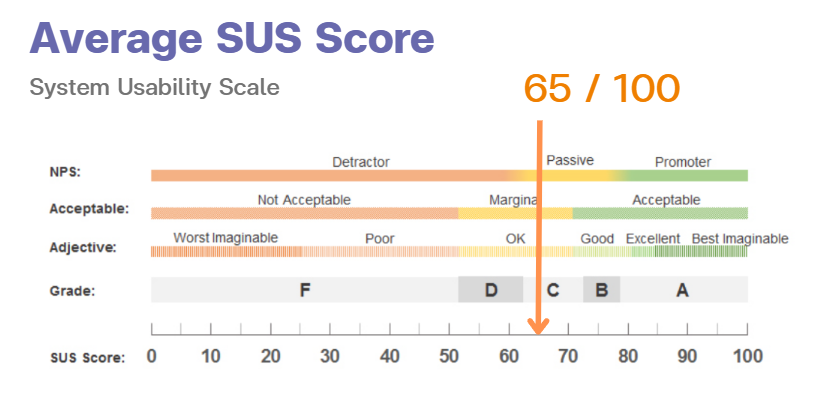
\includegraphics[width=0.60\textwidth,height=0.50\textheight,keepaspectratio]{SUST.png}
        \caption{คะแนน System Usability Scale (SUS Score) ของกลุ่ม Stakeholders}
        \label{fig:SUS score}
    \end{figure}
    \item \textbf{Technology Acceptance Model (TAM) - Perceived Usefulness (PU):} ประเมินการรับรู้ถึงประโยชน์ของระบบ 
    ว่าข้อมูลจากแบบจำลองช่วยเพิ่มประสิทธิภาพในการตัดสินใจวางแผนการเดินรถได้เพียงใด โดยมีข้อคำถามดังนี้
    \begin{itemize}
        \item ระบบนี้ช่วยให้ท่านทำงานได้รวดเร็วขึ้น
        \item ระบบนี้ช่วยปรับปรุงประสิทธิภาพการทำงานของท่าน
        \item ระบบนี้ช่วยท่านสามารถจัดการงานให้ปริมาณที่มากขึ้น
        \item ระบบนี้ช่วยเพิ่มความสำเร็จในการทำงานของท่าน
        \item ระบบนี้ช่วยให้ท่านทำงานได้ง่ายขึ้น
        \item ระบบนี้ช่วยให้ท่านปฏิบัติงานในหน้าที่ได้ง่ายขึ้น
    \end{itemize}
    ให้คะแนนระดับความเห็นด้วย เช่น 1 = ไม่เห็นด้วยอย่างมาก 5 = เห็นด้วยอย่างมาก
    โดยคำนวณค่าเฉลี่ยของคะแนนในส่วนนี้ได้ 4.595 ซึ่งอยู่ในระดับสูงมาก แสดงให้เห็นว่าผู้ใช้งาน
    รับรู้ถึงประโยชน์ของระบบจำลองในการช่วยเพิ่มประสิทธิภาพการตัดสินใจวางแผนการเดินรถได้อย่างชัดเจน
    \begin{figure}[H]
        \centering
        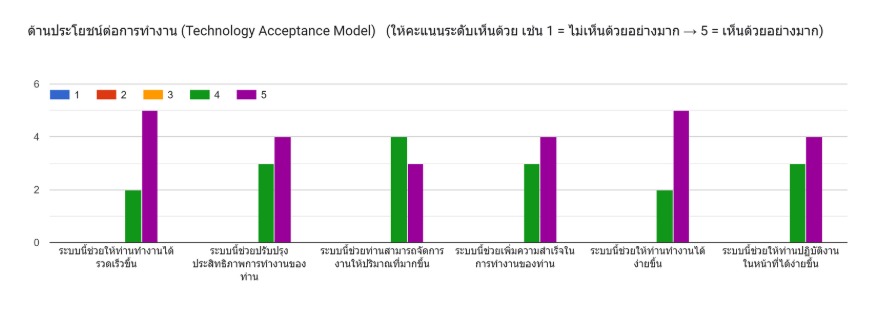
\includegraphics[width=0.60\textwidth,height=0.50\textheight,keepaspectratio]{TAMPU.png}
        \caption{คะแนน Technology Acceptance Model (TAM) - Perceived Usefulness (PU) ของกลุ่ม Stakeholders}
        \label{fig:TAM PU}
    \end{figure}

    \item \textbf{Overall Satisfaction:} ความพึงพอใจในภาพรวมต่อผลลัพธ์ที่ได้จากระบบ DeSS-T 
    โดยให้คะแนนระดับความพึงพอใจ เช่น 1 = ไม่พึงพอใจอย่างมาก 5 = พึงพอใจอย่างมาก
    โดยคำนวณค่าเฉลี่ยของคะแนนในส่วนนี้ได้ 4.43 แสดงให้เห็นว่าผู้ใช้งานมีความพึงพอใจในภาพรวมต่อผลลัพธ์ที่ได้จากระบบจำลอง DeSS-T อยู่ในระดับสูง
    \begin{figure}[H]
        \centering
        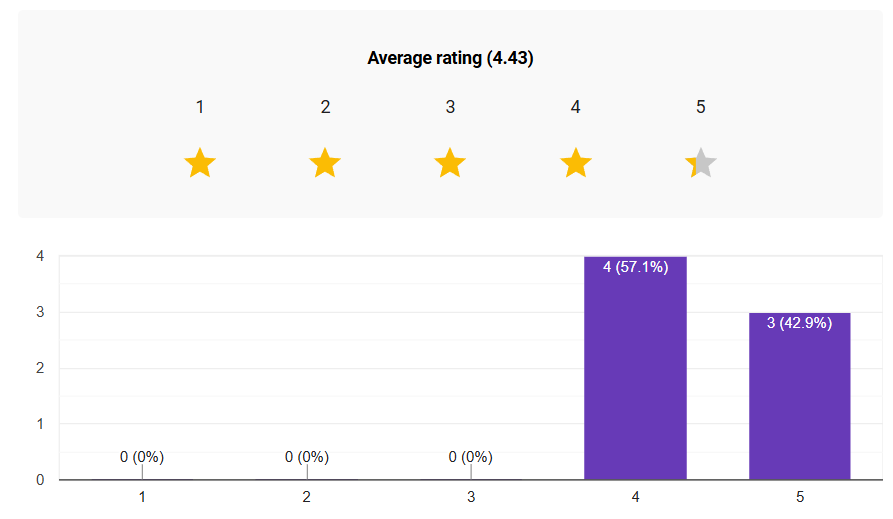
\includegraphics[width=0.60\textwidth,height=0.50\textheight,keepaspectratio]{overallT.png}
        \caption{คะแนน Overall Satisfaction ของกลุ่ม Stakeholders}
        \label{fig:Overall Satisfaction}
    \end{figure}

\end{itemize}

\textbf{ผลลัพธ์และวิเคราะห์เหตุผล:}
จากผลการทดสอบพบว่ากลุ่ม Stakeholders 
\subsection{การประเมินสำหรับบุคคลทั่วไป (General Users)}
\begin{mypara}
    \indent กลุ่มนี้ประกอบด้วยนักศึกษาและบุคคลทั่วไปโดยเน้นการประเมินด้านส่วนติดต่อผู้ใช้ (UI) และประสบการณ์การใช้งาน (UX) ผ่านเกณฑ์ดังนี้
\end{mypara}

\begin{itemize}
    \item \textbf{System Usability Scale (SUS Score):} วัดความยากง่ายในการใช้งานระบบโดยรวม 
    เพื่อดูว่าเครื่องมือที่มีความซับซ้อนต่อการใช้งานมากน้อยเพียงใด โดยมีข้อคำถามดังนี้
    \begin{itemize}
        \item ท่านต้องการกลับมาใช้งานระบบนี้อีก
        \item ท่านพบว่าระบบมีความซับซ้อนเกินจำเป็น
        \item ระบบง่ายต่อการใช้งาน
        \item ท่านต้องได้รับการความช่วยเหลือทางเทคนิคจึงจะสามารถใช้ระบบนี้ได้
        \item ฟังก์ชันในระบบทำงานได้อย่างราบรื่น
        \item ฟังก์ชันในระบบมีการทำงานสอดคล้องกัน
        \item ท่านคิดว่าคนส่วนใหญ่สามารถเรียนรู้การใช้งานระบบนี้ได้
        \item ระบบมีความยุ่งยากในการใช้งาน
        \item ท่านมีความมั่นใจขณะใช้งานระบบนี้
        \item ท่านจำเป็นต้องศึกษาอย่างมากก่อนใช้งานระบบนี้
    \end{itemize}
    ให้คะแนนระดับความเห็นด้วย เช่น 1 = ไม่เห็นด้วยอย่างมาก 5 = เห็นด้วยอย่างมาก
    โดยคำนวณคะแนน SUS Score ตามสูตรได้ผลลัพธ์อยู่ที่ 62.27 ซึ่งอยู่ในระดับปานกลาง
    แสดงให้เห็นว่าระบบมีความซับซ้อนในการใช้งานและอาจต้องใช้เวลาในการเรียนรู้ก่อนที่
    จะใช้งานได้อย่างคล่องตัว
    \begin{figure}[H]
        \centering
        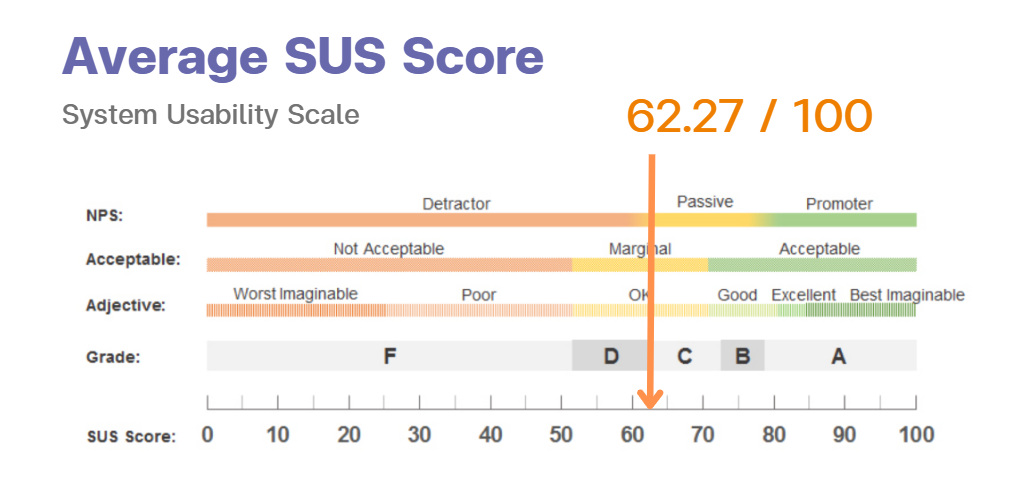
\includegraphics[width=0.60\textwidth,height=0.50\textheight,keepaspectratio]{SUS.png}
        \caption{คะแนน System Usability Scale (SUS Score) ของกลุ่มบุคคลทั่วไป}
        \label{fig:SUS score general}
    \end{figure}
    \item \textbf{UI/UX Heuristic Usability Test Score:} วัดผลตามหลักการออกแบบ 10 ประการ (Heuristics) 
    โดยมีข้อคำถามดังนี้
    \begin{itemize}
        \item ระบบมีการแสดงสถานะการใช้งานให้ผู้ใช้ทราบ
        \item ท่านสามารถเข้าใจภาษาและสัญลักษณ์ในระบบได้
        \item ท่านสามารถควบคุมระบบได้อย่างอิสระ
        \item ทั้งระบบมีการใช้มาตรฐานในการออกแบบแบบเดียวกัน
        \item ระบบมีการยืนยันเพื่อป้องกันไม่ให้เกิดข้อผิดพลาด
        \item ท่านรู้สึกคุ้นเคยกับการใช้งานระบบหรือไม่
        \item ระบบมีคีย์ลัดในการใช้งาน
        \item ระบบมีการออกแบบที่ ดูสวยงาม สบายตา
        \item ระบบมีคำอธิบายเมื่อเกิดข้อผิดพลาด
        \item ระบบมีคู่มือการใช้งานที่ชัดเจน
    \end{itemize}
    ให้คะแนนระดับความเห็นด้วย เช่น 1 = ไม่เห็นด้วยอย่างมาก 5 = เห็นด้วยอย่างมาก
    โดยคำนวณค่าเฉลี่ยของคะแนนในส่วนนี้ได้ 4.02 ซึ่งอยู่ในระดับดี แสดงให้เห็นว่าผู้ใช้งานมีความพึงพอใจ
    ต่อการออกแบบส่วนติดต่อผู้ใช้ (UI) และประสบการณ์การใช้งาน (UX) ของระบบจำลอง
     DeSS-T 
    \begin{figure}[H]
        \centering
        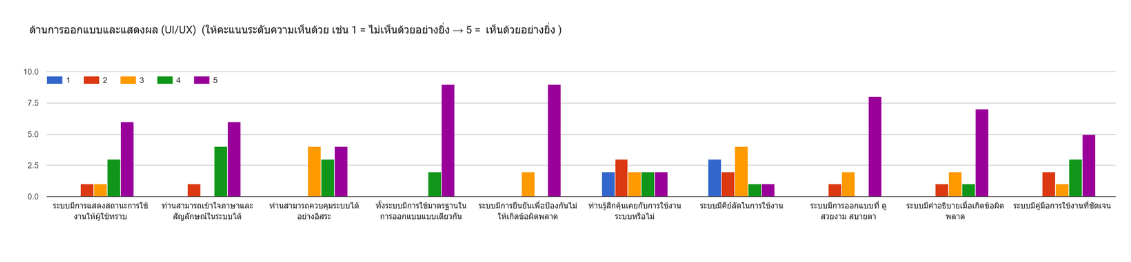
\includegraphics[width=0.60\textwidth,height=0.50\textheight,keepaspectratio]{UXUI.png}
        \caption{คะแนน UI/UX Heuristic Usability Test ของกลุ่มบุคคลทั่วไป}
        \label{fig:UIUX score general}
    \end{figure} 
    \item \textbf{Overall Satisfaction:} ความพึงพอใจในภาพรวมต่อผลลัพธ์ที่ได้จากระบบ DeSS-T 
    โดยให้คะแนนระดับความพึงพอใจ เช่น 1 = ไม่พึงพอใจอย่างมาก 5 = พึงพอใจอย่างมาก
    โดยคำนวณค่าเฉลี่ยของคะแนนในส่วนนี้ได้ 4.45 แสดงให้เห็นว่าผู้ใช้งานมีความพึงพอใจ
    ในภาพรวมต่อผลลัพธ์ที่ได้จากระบบจำลอง DeSS-T อยู่ในระดับสูง
    \begin{figure}[H]
        \centering
        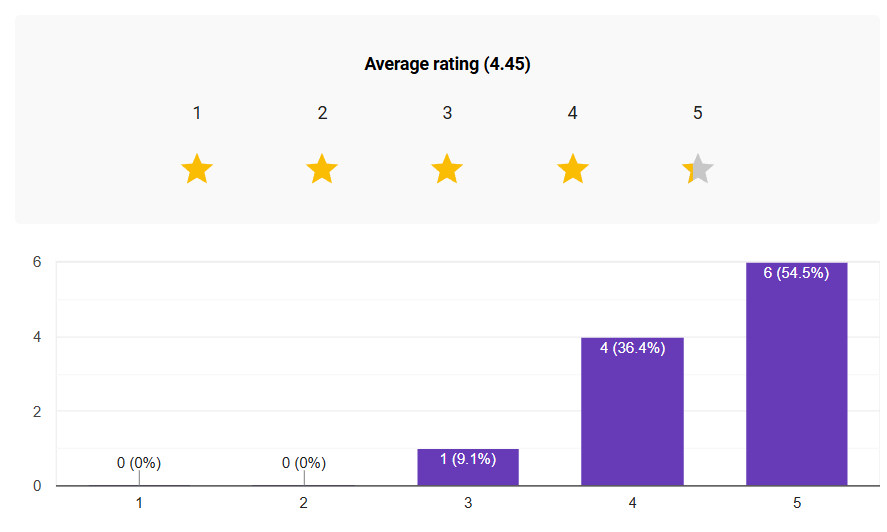
\includegraphics[width=0.60\textwidth,height=0.50\textheight,keepaspectratio]{overall.png}
        \caption{คะแนน Overall Satisfaction ของกลุ่มบุคคลทั่วไป}
        \label{fig:Overall Satisfaction general}
    \end{figure}
\end{itemize}

\textbf{ผลลัพธ์และวิเคราะห์เหตุผล:}
\indent จากผลการประเมินประสิทธิภาพและพึงพอใจของทั้งสองกลุ่ม สามารถวิเคราะห์ประเด็นสำคัญได้ดังนี้
\begin{enumerate}
\item \textbf{กลุ่มผู้ใช้งานที่เกี่ยวข้องกับการขนส่งสาธารณะ (Stakeholders):} 
พบว่าแม้คะแนน SUS Score จะอยู่ในระดับปานกลาง (65 คะแนน) ซึ่งสะท้อนถึงความซับซ้อน
ของระบบแต่ในทางกลับกัน คะแนนการรับรู้ประโยชน์ (TAM - PU) กลับสูงมากถึง 4.595
 และความพึงพอใจโดยรวมอยู่ที่ 4.43 วิเคราะห์ได้ว่า สำหรับผู้ที่มีเป้าหมายการใช้งานที่ชัดเจน 
 ความซับซ้อนของระบบถือเป็นข้อแลกเปลี่ยนที่คุ้มค่า (Trade-off) กับผลลัพธ์เชิงสถิติที่แม่นยำ 
 ซึ่งช่วยให้การวางแผนเดินรถมีประสิทธิภาพและรวดเร็วกว่าวิธีการดั้งเดิมอย่างเห็นได้ชัด

\item \textbf{กลุ่มบุคคลทั่วไป (General Users):} ผลการประเมินมีทิศทางที่น่าสนใจ 
โดยกลุ่มนี้ให้คะแนน SUS Score ต่ำที่สุด (62.27 คะแนน) แม้จะชื่นชมการออกแบบ UI/UX 
ในระดับดี (4.02) ก็ตาม วิเคราะห์เหตุผลได้ว่าเนื่องจากระบบ DeSS-T เป็นเครื่องมือเฉพาะทาง 
(Specialized Tool) ที่มีบริบทด้านการวางแผนขนส่งมวลชน ทำให้บุคคลทั่วไปที่ไม่มีความรู้พื้นฐาน
ในโดเมนนี้รู้สึกว่าระบบใช้งานยากและซับซ้อนเกินความจำเป็น หรือรู้สึกเข้าไม่ถึงฟังก์ชันเชิงลึก 
ส่งผลให้คะแนนความง่ายในการใช้งานลดต่ำลงเมื่อเทียบกับกลุ่มที่มีความเชี่ยวชาญ

\indent โดยสรุป แม้ระบบ DeSS-T จะมีความซับซ้อนในการเรียนรู้ช่วงแรก (Learning Curve)
 แต่คะแนนความพึงพอใจโดยรวมที่สูงกว่า 4.4 จากทั้งสองกลุ่ม ยืนยันว่าระบบสามารถทำหน้าที่
 เป็นเครื่องมือสนับสนุนการตัดสินใจที่ทรงประสิทธิภาพ โดยความซับซ้อนที่พบนั้นสอดคล้องกับความ
 สามารถในการคำนวณสถิติเชิงลึกที่ระบบมอบให้แก่ผู้ใช้งาน
\end{enumerate}

    \subsection{การรับข้อเสนอแนะการใช้งานระบบจำลอง}
        \begin{mypara}
            \indent โดยจะมีให้ผู้ใช้งานทำแบบสอบถามการทำงานของใช้งานได้อย่างถูกต้องหรือไม่
            พร้อมให้เสนอแนะของการปรับปรุงของแต่ละส่วนในระบบจำลองโดยจะมีหัวข้อในการสอบถาม ดังนี้
            \begin{itemize}
                \item ฟังก์ชันใดของระบบที่ท่านคิดว่าควรปรับปรุง  
                \item ท่านต้องการให้ระบบเพิ่มฟังก์ชันอะไร  
                \item ข้อเสนอแนะเพิ่มเติม  
            \end{itemize}
            \indent จากการรวบรวมข้อคิดเห็นจากกลุ่มผู้ใช้งานทั่วไปและผู้มีส่วนเกี่ยวข้อง 
            ได้ทำสรุปแนวทางจากการแนะนำเพื่อนำไปพัฒนาได้ดังนี้

            \begin{itemize}
                \item \textbf{การพัฒนาสื่อการเรียนรู้ด้วยตนเอง:} พัฒนาระบบแนะนำการใช้งาน 
                และจัดเตรียมไฟล์ตัวอย่างข้อมูลที่ระบุรูปแบบที่ชัดเจน เพื่อช่วยให้ผู้ใช้รายใหม่สามารถใช้งานระบบได้
                โดยไม่ต้องมีผู้เชี่ยวชาญให้คำแนะนำตัวต่อตัว
                \item \textbf{การปรับปรุงความลื่นไหลของส่วนติดต่อผู้ใช้ (UI/UX):} พัฒนาระบบแสดงสถานะการทำงาน (Progress Bar), 
                ฟังก์ชันการแสดงข้อมูลเมื่อวางเมาส์เหนือจุดจอด (Hover Info), และปรับปรุง Layout ให้รองรับหน้าจอทุกขนาด (Responsive Design)
                \item \textbf{การเพิ่มปัจจัยด้านสภาพแวดล้อมจำลอง:} บูรณาการปัจจัยด้านความหนาแน่นของการจราจร (Traffic Conditions)
                 และสภาพการณ์จำลองกรณีเกิดเหตุฉุกเฉินบนท้องถนน เพื่อให้ผลลัพธ์จากการจำลองมีความสมจริงยิ่งขึ้น
                \item \textbf{การเพิ่มเสถียรภาพในการจัดการข้อมูล:} ปรับปรุงระบบการจัดการไฟล์ (Save/Load Data) ให้มีความเสถียร 
                ลดโอกาสการเกิด Error ขณะนำเข้าหรือบันทึกข้อมูล และแก้ไขข้อผิดพลาดในส่วนของการรับข้อมูลนำเข้า (Input Validation)
            \end{itemize}
        \end{mypara}


